\chapter{Introduksjon}


\section{Om applikasjonen}
\begin{itemize}
\item All kode i applikasjonen er på engelsk med hensikt til at denne skal eventuelt kompileres på forskjellige miljøer med ulike typer \"encoding\". 
\item Kompilert med SDK versjon 23: Android 6.0 Marchmallow, Build tools: 23.0.0
\item Mål SDK: API 21: Android 5.0 (Lollipop) Minimal SDK: API 19: Android 4.4 (KitKat)
\item ID for applikasjonen: com.example.s198569.hangman
\item Utviklingsmiljø: Android Tools 1.3.2, Fedora Linux 22 x64
\item Debugging og testing gjennomført på LGE Optimus 2X (P990) med Cyanogenmod Android 4.4.4. Enheten har samme skjermstørrelse som målenhet Samsung Nexus S.
\end{itemize}


\section{Hva har jeg lært meg}
Jeg har aldri før utviklet for Android derfor er alle komponenter som jeg bruker i applikasjonen nye for meg. Jeg hatt som mål å strekke meg noe utøver de krav som er beskrevet i oppgavebeskrivelsen. Følgende liste er et sammendrag over de komponenter som er implementert i applikasjonen utøver de som vært introdusert i forelesningene:
\begin{enumerate}
\item Lagring og lesing av data i appens interne \texttt{SQLite} database.
\item Endring og  av komponenter. Eksempel på dette er egne stiler som er brukt i f.eks. \texttt{GamePlayActivity} der det er opprettet egne stiler både for knapper og \texttt{EditText} som benyttes til å vise ord som skal gjettes.
\item Bruk av \texttt{PreferanceActivity} for å vise innstillinger for applikasjonen på en oversiktlig og ryddig måte. 
\item Opprette grafiske komponenter på en dynamisk måte. Eksempel på dette er tastatur som blir satt opp avhengig av det språk som er valgt for systemet eller applikasjonen (tastaturet blir satt opp fra et predefinert xml fil som inneholder alle bokstaver fra det språket). 
\item Endre språk i applikasjonen uten at språk for systemet blitt endret. Det valgte språket blir også bevart dersom applikasjonen roteres. 
\end{enumerate}



\chapter{Bruksanvisning}
I følgende kapittel beskrives det hvordan det er tenkt at spillet skal brukes samt en enkel navigasjon mellom applikasjonens skjermbilder. 

\section{Oppstart av applikasjonen}
Når applikasjonen startes blir brukeren presentert av skjermbilde presentert i figur \ref{fig:activity_front}. 
\begin{figure}[ht]
\centering
 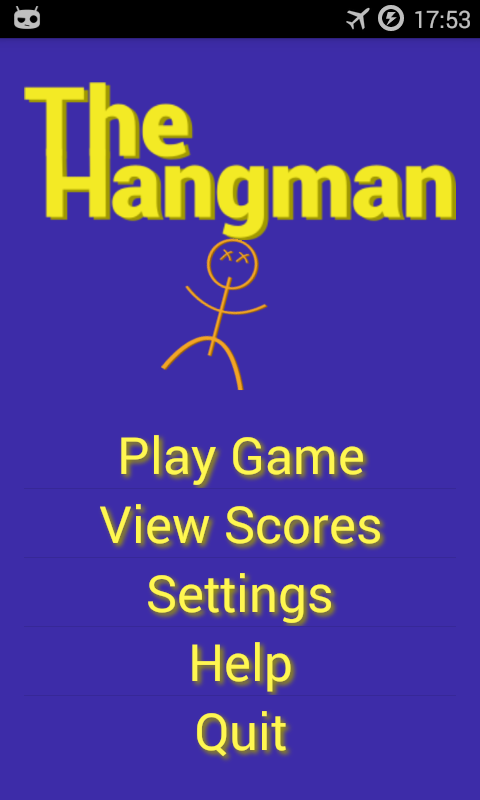
\includegraphics[scale=0.25]{./img/bruksanvisning/1.png}
 \caption{Startskjerm.}
 \label{fig:activity_front}
\end{figure}

Fra dette bilde er det mulig for spilleren å: 
\begin{description}
\item[Play Game] Starte nytt spill. Dette vil ta spilleren til neste skjermbilde der det er mulig å registrere en ny spiller eller velge allerede eksisterende spillere som er registrert fra før.
\item[View Scores] Se på en sammenstilling av poeng for registrerte spillere. Sammenstillingen er sortert etter total poengsum synkende.
\item[Settings] Innstillinger for appen som valg av språk og lyd på eller av (lydeffekter er ikke implementert ennå).
\item[Help] Skjermbilde med regler for applikasjonen informasjon om applikasjonen. 
\item[Quit] Avlutter applikasjonen. 
\end{description}


\section{Nytt spill}

Spilleren blir presentert med et skjermbilde for å starte nytt spill , figur \ref{fig:registrering}. Her er det mulig å starte et nytt spill gjennom å registrere en ny spiller eller fortsette som en spiller som allerede er registrert fra før. Figur \ref{fig:ny_spiller} viser tilnærming for registrering av en ny spiller. Her blir brukeren varslet om at et nytt brukernavn er registrert via en \texttt{toast} og spurt dersom man ønsker å fortsette å spille med den nye spilleren. Spillet starter og et nytt brukernavn er presenter på spille aktiviteten i nord-vestre hjørne , figur \ref{fig:spill_igang}.

\begin{figure}[ht]
    \centering
    \begin{subfigure}[b]{0.3\textwidth}
        
\includegraphics[width=\textwidth]{./img/bruksanvisning/2.png}
        \caption{Registrering.}
        \label{fig:registrering}
    \end{subfigure}
    \begin{subfigure}[b]{0.3\textwidth}
        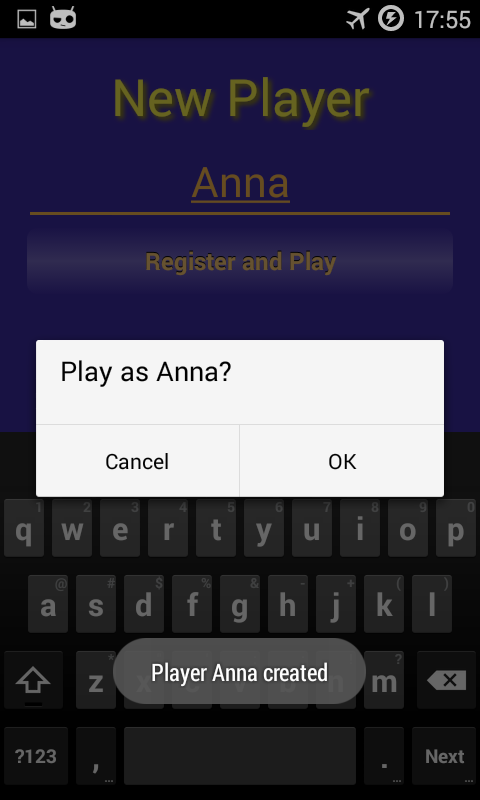
\includegraphics[width=\textwidth]{./img/bruksanvisning/3.png}
        \caption{Ny spiller registrert.}
        \label{fig:ny_spiller}
    \end{subfigure}
    \begin{subfigure}[b]{0.3\textwidth}
        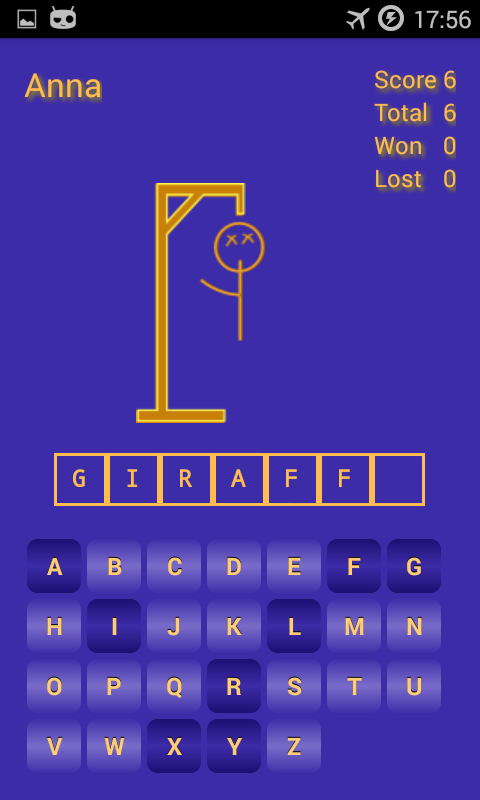
\includegraphics[width=\textwidth]{./img/bruksanvisning/4.png}
        \caption{Pågående spill}
        \label{fig:spill_igang}
    \end{subfigure}
    \caption{Nytt spill med en ny spiller}\label{fig:new_game_activities}
\end{figure}

Etter et spilleren har gjettet alle ord og vunnet eller ha misslykket med å avsløre hvilket ord som skjler seg bak firkantene blir spilleren spurt om man ønsker å spille én gang til, figur \ref{fig:fortsette}. Dersom det svares ja startes et nytt spill i samme økt. Dersom man har spilt minst et spill i økten blir spilleren presentert med enkel statistikk for den pågående økten i nord-østlig hjørne, se figur \ref{fig:nyt_spill_samme_okt}. I statistikken presenteres: (1) aktuelt antall poeng, (2) totalt antall poeng som spilleren har tjent sammen i pågående økt, (3) antall spill som er vunnet i økten samt (4) antall spill som er tapt. 

\begin{figure}[ht]
    \centering
    \begin{subfigure}[b]{0.3\textwidth}
        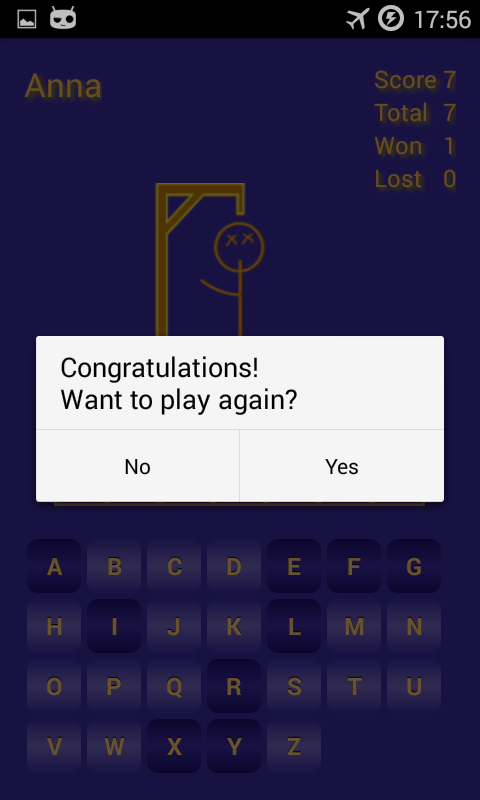
\includegraphics[width=\textwidth]{./img/bruksanvisning/5.png}
        \caption{Fortsette?}
        \label{fig:fortsette}
    \end{subfigure}
    \begin{subfigure}[b]{0.3\textwidth}
        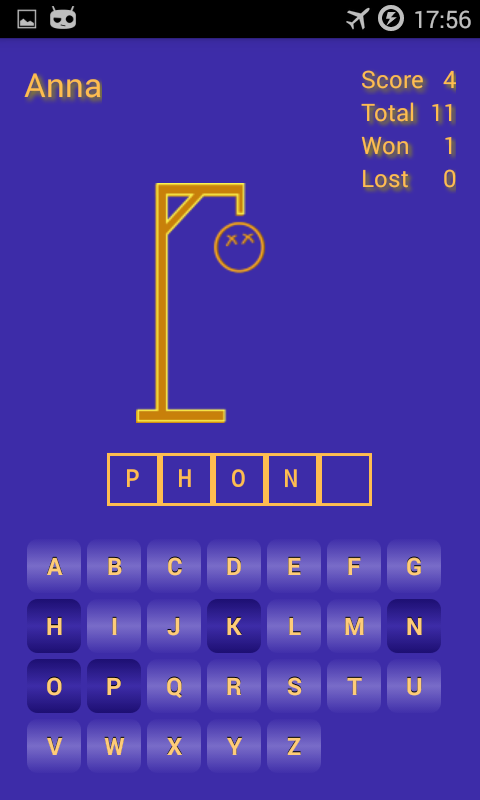
\includegraphics[width=\textwidth]{./img/bruksanvisning/6.png}
        \caption{Nytt spill.}
        \label{fig:nyt_spill_samme_okt}
    \end{subfigure}
    \caption{Nytt spill i samme økt.}\label{fig:new_game_activities}
\end{figure}

\section{Innstillinger}





\chapter{Arkitektur og struktur}

\chapter{Kode og løsninger}

\section{Lagring av brukerdata}
Lagring av brukerdata på enheten blir foretatt gjennom bruk av SQLite database. 

\chapter{Utfordringer}
\section{Rotasjon}
Her skal man forklare forskjellen mellom å lagre status av skjermen på den gamle måten og den nye i systemet. Hvordan de forskjellige komponentene lastes om. 
\begin{lstlisting}[language=Java]
    @Override
    protected void onSaveInstanceState(Bundle outState) {
        super.onSaveInstanceState(outState);

        outState.putString(PLAYERNAME, pName);
        outState.putInt(LETTERSCOUNT, lettersCount);
        outState.putCharArray(LETTERS, letters);
        outState.putInt(GAMESCORE, gameScore);
        outState.putInt(SESSIONSCORE, sessionScore);
        outState.putInt(TRYCOUNT, tryCount);
        outState.putInt(LETTERSGUESSED, lettersGuessed);
        outState.putInt(GAMESWON, gamesWon);
        outState.putInt(GAMESLOST, gamesLost);

        Toast.makeText(this, "Data er lagret", Toast.LENGTH_SHORT).show();

    }
\end{lstlisting}

\begin{lstlisting}
 @Override
    protected void onRestoreInstanceState(Bundle savedInstanceState) {
        super.onRestoreInstanceState(savedInstanceState);


        pName = savedInstanceState.getString(PLAYERNAME);
        lettersCount = savedInstanceState.getInt(LETTERSCOUNT);
        letters = savedInstanceState.getCharArray(LETTERS);
        gameScore = savedInstanceState.getInt(GAMESCORE);
        sessionScore = savedInstanceState.getInt(SESSIONSCORE);
        tryCount = savedInstanceState.getInt(TRYCOUNT);
        lettersGuessed = savedInstanceState.getInt(LETTERSGUESSED);
        gamesWon = savedInstanceState.getInt(GAMESWON);
        gamesLost = savedInstanceState.getInt(GAMESLOST);

        updateHangmanImage();
        Toast.makeText(this, "Restoring game score: "+gameScore, Toast.LENGTH_SHORT).show();

        playerName.setText(pName);
        gameScoreView.setText(String.valueOf(gameScore));
        sessionScoreView.setText(String.valueOf(sessionScore));
        gameScoreView.setText(String.valueOf(gamesWon));
        sessionScoreView.setText(String.valueOf(sessionScore));
    }
\end{lstlisting}

\section{SQLite}

\chapter{Lagring av data}

